\documentclass[12pt,a4paper]{article}
\usepackage[utf8]{inputenc}
\usepackage{graphicx}
\usepackage{geometry}
\usepackage{enumitem}
\usepackage{titlesec}
\usepackage{hyperref}

\geometry{margin=2.5cm}

\title{Regional Analysis}
\date{}

\begin{document}

\maketitle

\section{Number of Students by Region}
Shiraz dominates with 193 students, accounting for more than half of the total student population (see Figure~\ref{fig:students-region}). Fars (excluding Shiraz) follows with 68 students. Other notable regions include: Unknown (40), Hormozgan (17), Bushehr (13). Very few students come from Kerman, Khuzestan, Abroad, Golestan, and Yazd (efwer than five each).

\begin{figure}[h!]
    \centering
    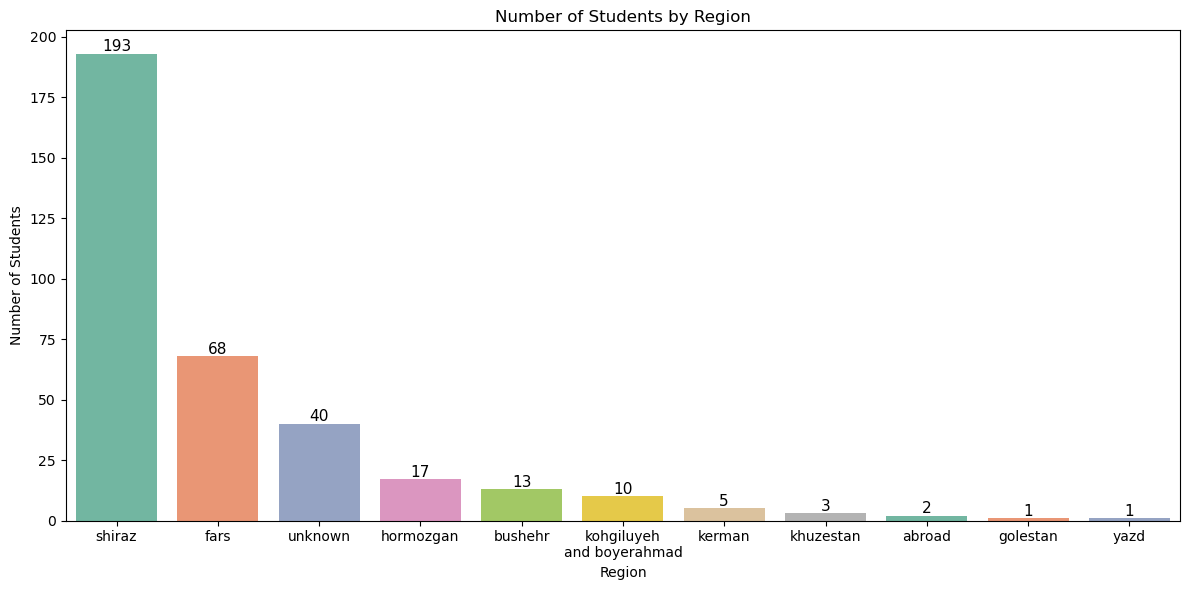
\includegraphics[width=0.95\textwidth]{Number of Students by Region.png}
    \caption{Number of Students by Region}
    \label{fig:students-region}
\end{figure}

\section{Total Income by Region}
Shiraz again leads significantly, generating over 11,064,300,000 IRR (11.1B IRR), which constitutes the majority of income (see Figure~\ref{fig:income-region}). Fars province contributes approximately 3,473,600,000 IRR (3.47B IRR), followed by Unknown (2.05B IRR), Hormozgan (0.84B IRR), and Bushehr (0.67B IRR). Other regions contribute minimally.

\begin{figure}[h!]
    \centering
    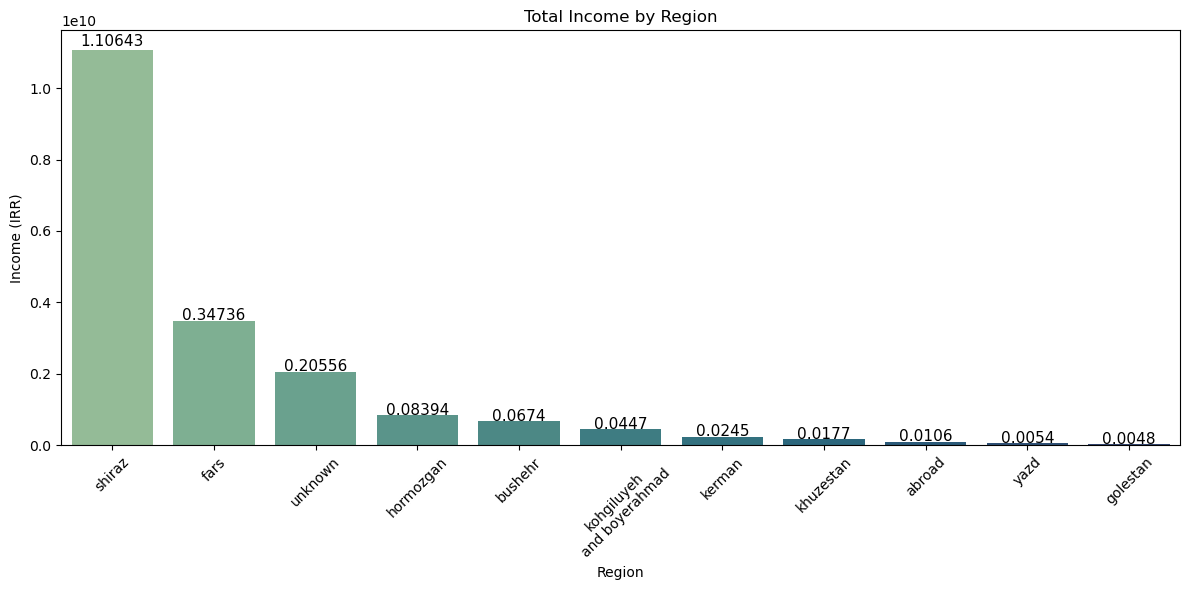
\includegraphics[width=1\textwidth]{Total Income by Region.png}
    \caption{Total Income by Region}
    \label{fig:income-region}
\end{figure}

\section{Income Share by Region (Top 5 Regions)}
According to Figure~\ref{fig:income-share}, Shiraz alone accounts for 57.7\% of total income. The next four regions are Fars (18.1\%), Unknown (10.7\%), Hormozgan (4.4\%), and Bushehr (3.5\%). Collectively, the top five regions contribute more than 94\% of the total income, while all other regions together account for only about 6\%.

\begin{figure}[h!]
    \centering
    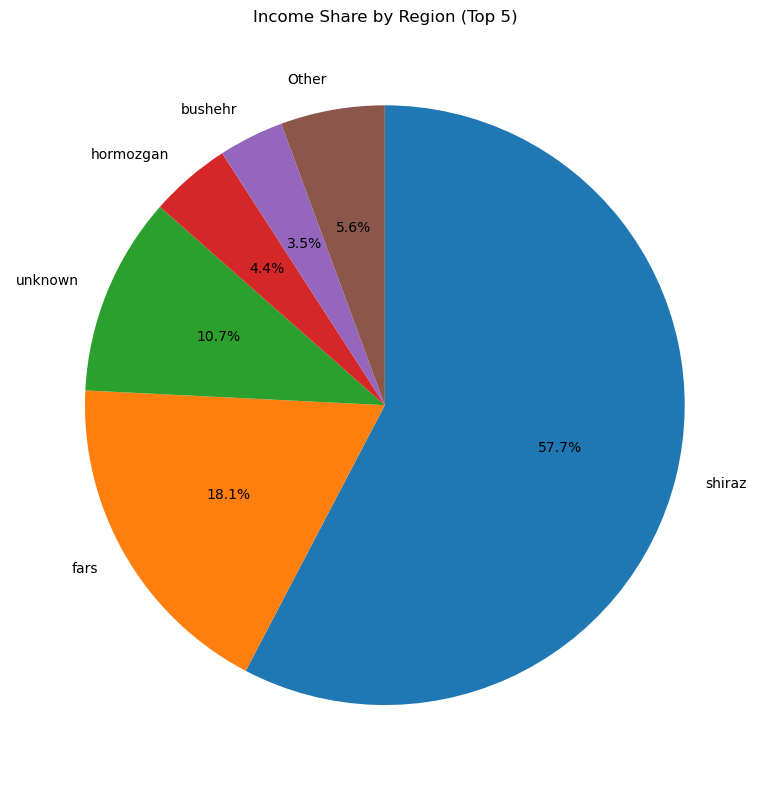
\includegraphics[width=0.8\textwidth]{Income Share by Region (Top 5) Pie Chart.png}
    \caption{Income Share by Region (Top 5)}
    \label{fig:income-share}
\end{figure}

\section{Number of Students in Each Region by Course Type}
Barista is the most popular course in Shiraz and Fars. Pizza, Burger, and Sausage courses also show up in multiple provinces. Traditional and Kabab courses appear only occasionally and remain largely localised (see Figure~\ref{fig:region-course}).

\begin{figure}[h!]
    \centering
    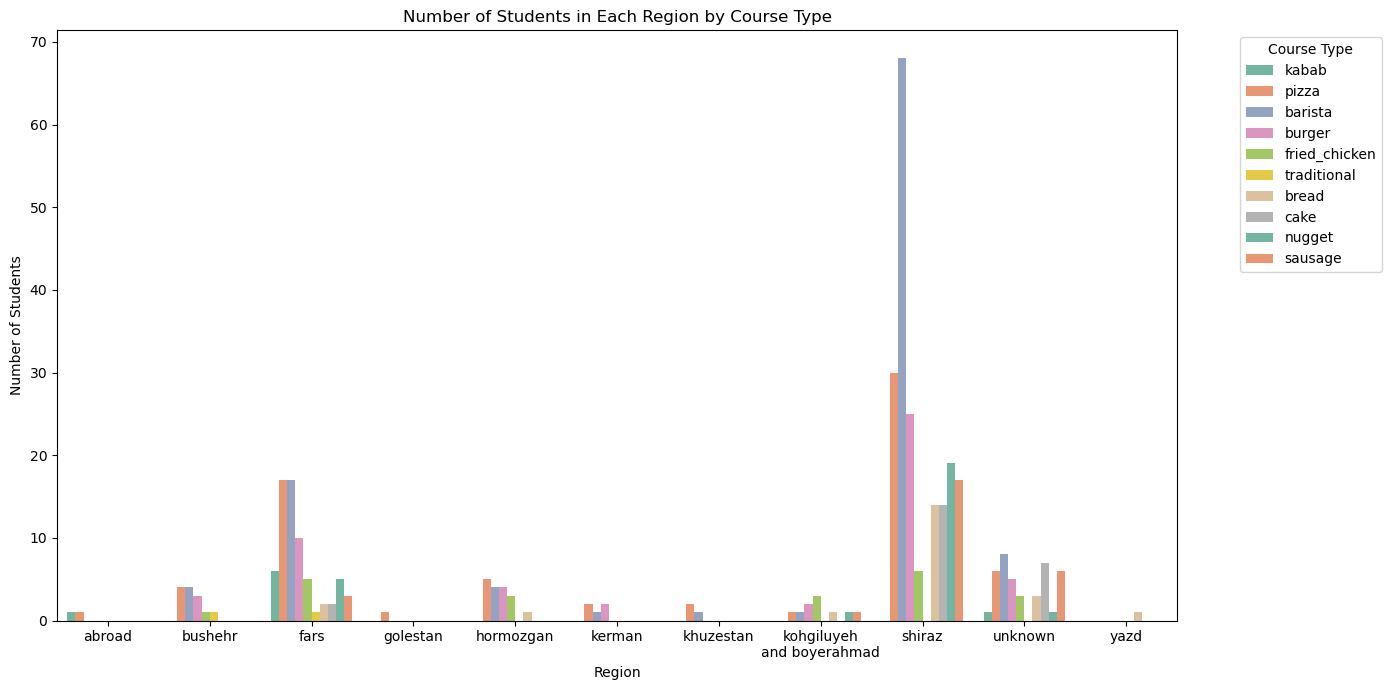
\includegraphics[width=1\textwidth]{Number of Students in Each Region by Course Type.png}
    \caption{Number of Students in Each Region by Course Type}
    \label{fig:region-course}
\end{figure}

\section{Number of Students in Each Region by Season}
Shiraz consistently has high enrolment across all four seasons, peaking in Summer and Autumn (see Figure~\ref{fig:region-season}). Fars also shows a seasonal distribution, though on a smaller scale. Seasonal spikes in other provinces are minimal.

\begin{figure}[h!]
    \centering
    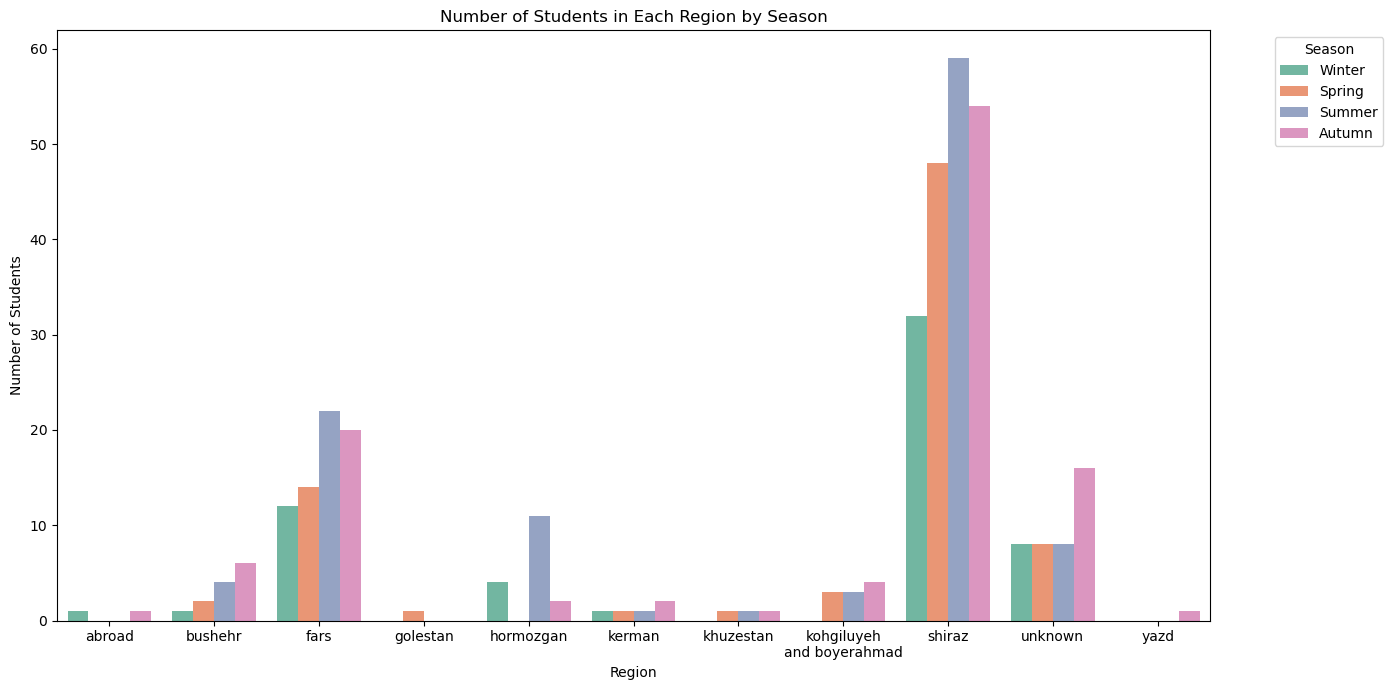
\includegraphics[width=1\textwidth]{Number of Students in Each Region by Season.png}
    \caption{Number of Students in Each Region by Season}
    \label{fig:region-season}
\end{figure}

\section*{Summary}
\begin{itemize}
    \item Shiraz is the core region in terms of student count and income.
    \item Most of the income comes from a few key regions.
    \item Opportunities exist in regional expansion, tailoring course offerings, and seasonal targeting.
    \item More visibility into regional preferences may help optimise outreach and scheduling.
\end{itemize}

\newpage
\section*{Recommendation} Expand marketing efforts beyond Shiraz and Fars to diversify income sources, while tailoring course offerings to match regional preferences.

\end{document}